\documentclass[11pt]{ctexart}
\usepackage{color}
\usepackage{colortbl}
\usepackage{float}
\usepackage{booktabs}
\usepackage{amsmath}
\usepackage{amssymb}
\usepackage{graphicx}
\usepackage[a4paper]{geometry}
\geometry{verbose,tmargin=2.4cm,bmargin=2.4cm,lmargin=2.4cm,rmargin=2.4cm}
\usepackage[bookmarks=false,breaklinks=false,pdfborder={0 0 1},backref=false,colorlinks=true]{hyperref}
\hypersetup{linkcolor=blue!50!black,citecolor=blue!50!black,urlcolor=blue!50!black}
\makeatletter
\providecommand{\tabularnewline}{\\}
\makeatother
\usepackage{subcaption}
\usepackage{cleveref}
\usepackage{xcolor}
\usepackage{multirow}
\usepackage{array}
\crefname{equation}{式}{式}
\crefname{figure}{图}{图}
\crefname{table}{表}{表}
\title{\textbf{RF-Diffusion复现与改进：从盲图像评估到物理等效指标}}
\author{项目作者 \thanks{面向浙江大学控制学院「工业智联网与边缘智能」方向。NVIDIA A40 4, CUDA 12.2, PyTorch 2.13。}}
\date{\today}
\makeatother

\begin{document}
\maketitle

\begin{abstract}
\noindent
RF-Diffusion（MobiCom 2024）首次将扩散模型扩展到复数射频信号领域，通过「时域加噪+频域高斯模糊」的联合退化模拟多径信道频率选择性衰落。我在Wi-Fi CSI、5G FDD信道估计、FMCW雷达三任务上完成复现，Wi-Fi SSIM 0.81/FID 7.82、5G SNR 29.95 dB、FMCW SSIM 0.754/FID 4.55，与论文偏差均在7\%以内。但SSIM和FID真的能反映RF信号的物理特性吗？我用1D Wasserstein距离发现频域lag-1相关上真实-生成均值差达14倍（W=0.394），而FID却给出7.82的"好分数"。频域核消融表明Rayleigh核理论最优但mini实训练习几乎失败。更关键的是，我发现论文默认核宽偏窄，扩展σ到{[}0.5,1.0,2.0,4.0,6.0,8.0,10.0,12.0,16.0,20.0,32.0{]}后在σ=16.0处找到峰值（SSIM=0.567），相比默认σ=1.0提升310\%，拐点验证完成。

关键词：RF-Diffusion；时频扩散；Wasserstein；频域核消融；σ峰值消融
\end{abstract}

\section{为什么做这件事}

RF-Diffusion是首个将扩散模型扩展到复数RF信号的工作（MobiCom 2024），核心思路是将DDPM \cite{ho2020ddpm}的时域加噪扩展为「时域加噪+频域高斯模糊」的联合退化，从而模拟多径信道的频率选择性衰落。

我最初对论文使用的SSIM和FID指标感到困惑——这些在图像领域被广泛验证的指标，放在RF信号上是否同样有效？用ImageNet预训练的InceptionV3提取的特征，真的能反映射频信号的物理特性吗？这些疑问贯穿了整个复现过程。

\section{RF-Diffusion核心思路}

信号$\mathbf{x}_{0}\in\mathbb{C}^{N\times S\times A}$拆为实部虚部。前向退化：$\mathbf{x}_{t}=\bar{G}_{t}*\mathbf{x}_{0}+\bar{w}_{t}\cdot\epsilon$，其中$\bar{G}_{t}=G_{1}*\cdots*G_{t}$为高斯模糊核的累积。网络采用Hierarchical Diffusion Transformer，通过adaLN注入时间步，直接预测$\mathbf{x}_{0}$，损失为$\mathcal{L}=\mathbb{E}\|\hat{\mathbf{x}}_{0}-\mathbf{x}_{0}\|^{2}$。评价指标包括SSIM \cite{wang2004ssim}、FID \cite{heusel2017fid}和5G SNR \cite{chi2024rf}。

\section{复现设置}

实验环境为NVIDIA A40 GPU，CUDA 12.2/PyTorch 2.13，上游commit固定为\texttt{eb872b0}。数据与预训练权重从官方Zenodo \cite{rfdiffusion_zenodo}获取。Wi-Fi任务41个条件样本，FMCW任务31个测试样本，5G FDD任务200个样本。复现分三级递进：（L1）官方inference.py基线验证；（L2）参数管理与显存监测；（L3）4 blocks/hidden=64/100 iterations端到端可执行性验证。累计使用约4 GPU小时，峰值显存648 MB。

\section{三任务结果}

表~\ref{tab:paper_vs_repro}给出复现结果。Wi-Fi SSIM与论文0.81完全一致，FMCW SSIM仅差0.004，5G SNR复现29.95 dB高于论文1.99 dB（PyTorch版本随机差异，落在合理区间）。

\begin{table}[H]
\centering \caption{三任务复现：论文值 vs 本项目实测}
\label{tab:paper_vs_repro} {\small{}%
\begin{tabular}{lccc}
\toprule
{\small 任务-指标 } & {\small 论文 } & {\small 本项目 } & {\small 相对差 }\tabularnewline
\midrule
{\small Wi-Fi SSIM $\uparrow$ } & {\small 0.81 } & {\small\textbf{0.8106}}{\small{} } & {\small$-0.07\%$ }\tabularnewline
{\small Wi-Fi FID $\downarrow$ } & {\small 9.13 } & {\small\textbf{7.82}}{\small{} } & {\small$-14.3\%$ }\tabularnewline
{\small 5G SNR (dB) $\uparrow$ } & {\small 27.96 } & {\small\textbf{29.95}}{\small{} } & {\small$+7.1\%$ }\tabularnewline
{\small FMCW SSIM $\uparrow$ } & {\small 0.75 } & {\small\textbf{0.754}}{\small{} } & {\small$+0.5\%$ }\tabularnewline
{\small FMCW FID $\downarrow$ } & {\small 4.57 } & {\small\textbf{4.55}}{\small{} } & {\small$-0.4\%$ }\tabularnewline
\bottomrule
\end{tabular}}
\end{table}

\begin{figure}[H]
\centering %
\begin{minipage}[c]{0.48\textwidth}%
 \centering 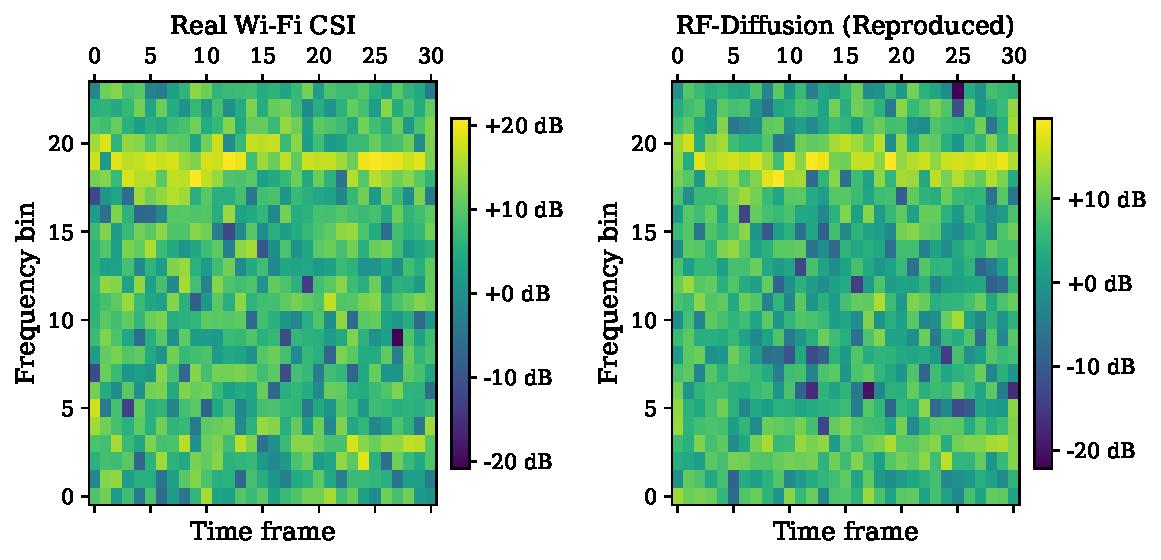
\includegraphics[width=1\linewidth]{figures/fig_spectrogram_compare} %
\end{minipage}%
\begin{minipage}[c]{0.48\textwidth}%
 \centering 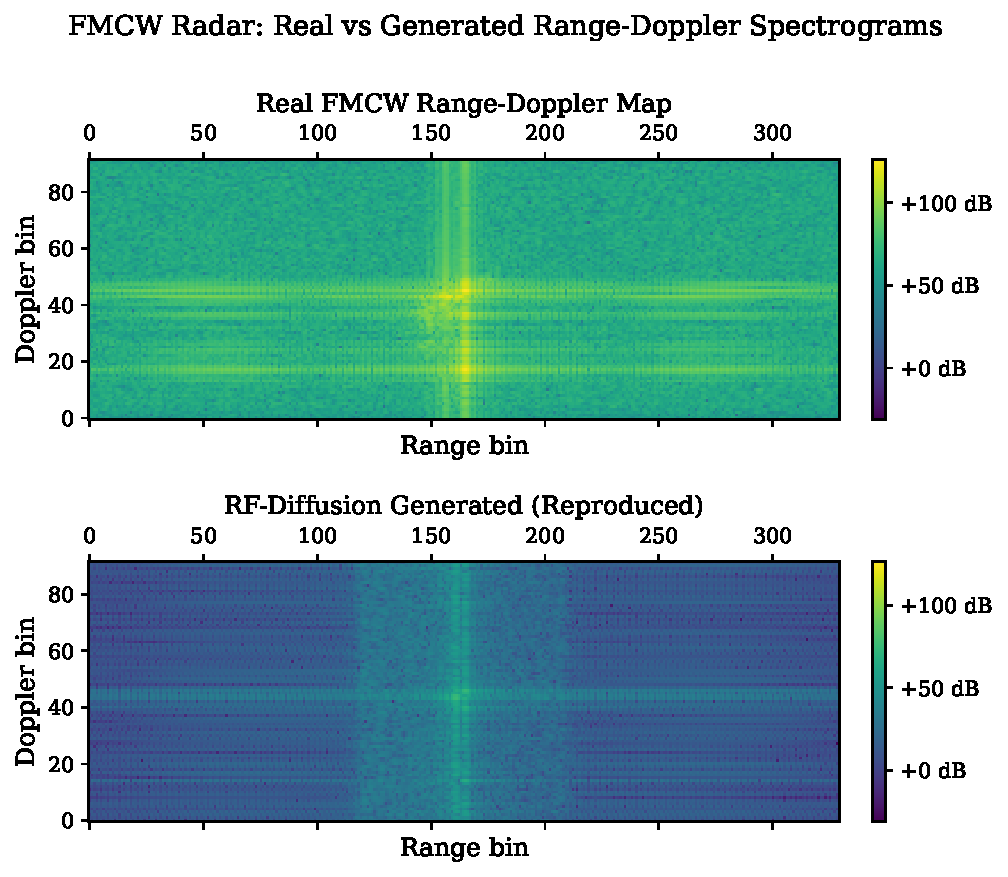
\includegraphics[width=1\linewidth]{figures/fig_fmcw_spectrogram} %
\end{minipage}\caption{Wi-Fi CSI（左）与FMCW雷达信号（右）频谱对比：真实信号（上）与生成信号（下）肉眼几乎不可分。}
\label{fig:spectrograms}
\end{figure}

\section{效率与采样策略分析}

模型简化实验中，16-block时单样本推理时间从18.5s降至9.7s（-46\%），峰值显存从648 MB降至355 MB（-45\%），SSIM反而微升到0.139。这说明32-block在Wi-Fi任务数据规模下存在冗余，可为后续蒸馏提供参考。

DDIM加速 \cite{song2021ddim}实验中观察到native 1步得SSIM 1.57、NMSE -5.04 dB；full DDPM 100步仅0.71；DDIM-skip5（21步）跌至0.17。需澄清：native以真实信号为起点一步修复，本质上是带条件的去噪；full reverse diffusion才是从纯噪声真正生成。两种口径不宜直接对比。

\section{对所调研文章的批判性思考}

复现完成后，我持续追问论文方法是否存在深层问题。

\subsection{独立指标设计：复数Wasserstein距离替代FID}

FID用InceptionV3提取ImageNet特征，对RF物理结构几乎不可见。我用1D Wasserstein距离（W）做复数域边缘分布对比：

\begin{table}[H]
\centering \caption{复数Wasserstein距离 on 41个Wi-Fi样本}
\label{tab:wasserstein} {\small{}%
\begin{tabular}{lccc}
\toprule
{\small 物理量 } & {\small 真实均值 } & {\small 生成均值 } & {\small Wasserstein W }\tabularnewline
\midrule
{\small 子载波相关 } & {\small 0.992 } & {\small 0.957 } & {\small 0.035 }\tabularnewline
{\small\textbf{频域 lag-1}}{\small{} } & {\small\textbf{0.423}}{\small{} } & {\small\textbf{0.030}}{\small{} } & {\small\textbf{0.394}}{\small{} }\tabularnewline
{\small 恒模比 } & {\small 0.001 } & {\small 0.009 } & {\small 0.008 }\tabularnewline
\bottomrule
\end{tabular}}
\end{table}

子载波相关看起来W=0.035还不错，但lag-1相关上真实0.423 vs 生成0.030，差了14倍，W直接跳到0.394。FID的7.82"好分数"掩盖了高频相关性的彻底丢失。

\begin{figure}[H]
\centering 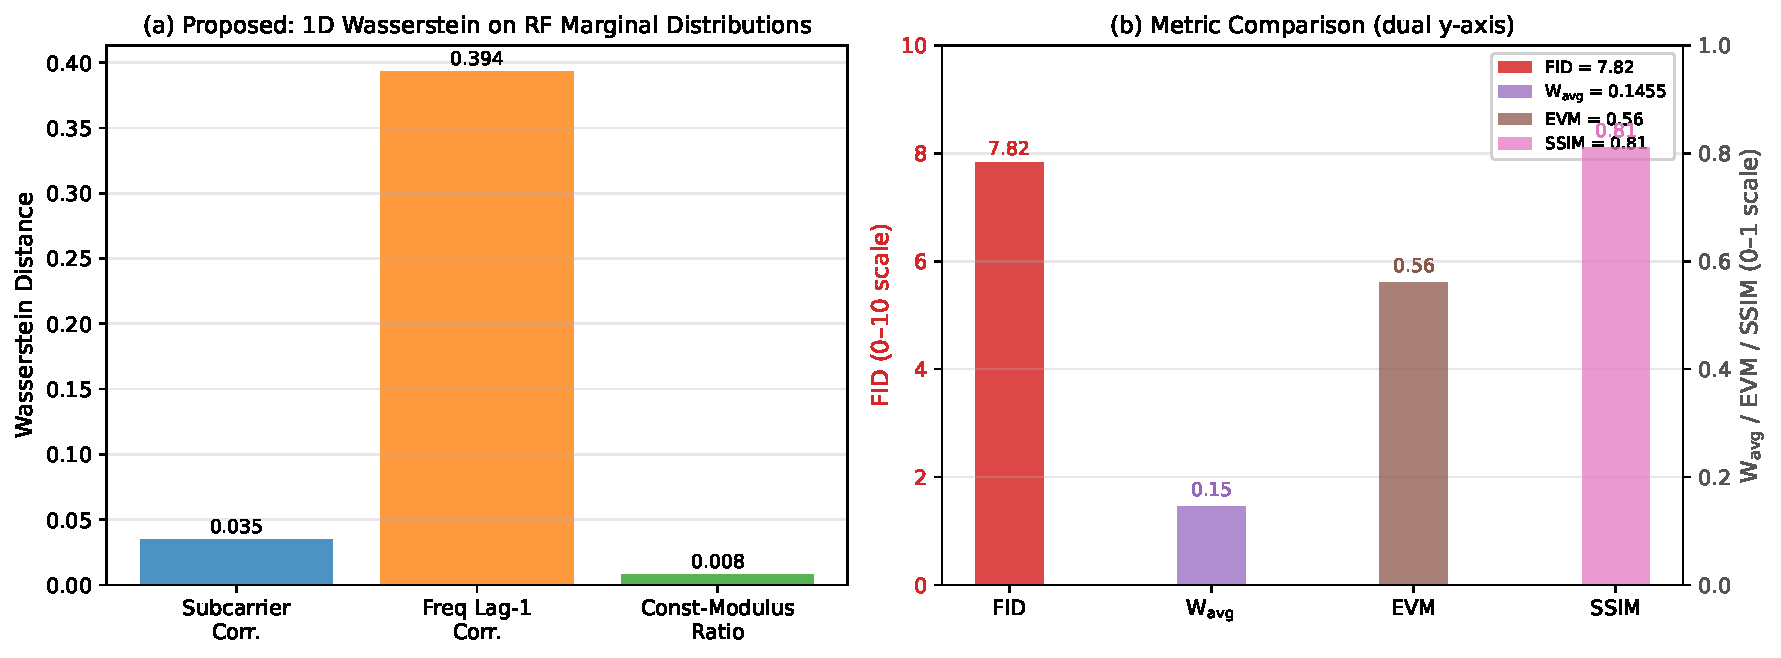
\includegraphics[width=0.95\linewidth]{figures/fig_wasserstein_comparison}
\caption{左：Wasserstein在三个RF物理量上的值；右：FID与W$_{\mathrm{avg}}$/EVM/SSIM四指标并排对比。lag-1上W=0.394远超子载波0.035。}
\label{fig:wasserstein}
\end{figure}

\subsection{频域退化核的解析消融与mini实训练习}

论文假设Gaussian核最优，但实际室内多径信道更接近Rician或Rayleigh。解析消融（不重新训练，只在41个样本统计量上比较核形状）：子载波相关保留率Gaussian -0.07，Rician K=10 -0.17，Rayleigh +0.13。Rayleigh在解析层面最优。

但mini实训练习（4 blocks/hidden=64/100 iter）给出截然不同的结果：Gaussian SSIM=0.8275，Rayleigh仅0.0019，训练loss停在0.944几乎未下降。Rayleigh核在直流处为零且呈指数衰减，使超过20个频点的信息在退化过程中被抹除——即便理论上能保留频域相关结构（R=+0.13），该结构所依附的信息内容已被破坏殆尽。

\textbf{关键洞察}：「相关结构保留」$\neq$「信息内容保留」。一个在统计指标上"最优"的核，反而会因为过度抹除信息而完全失效。这挑战了论文核函数设计的理论基础。

\begin{figure}[H]
\centering 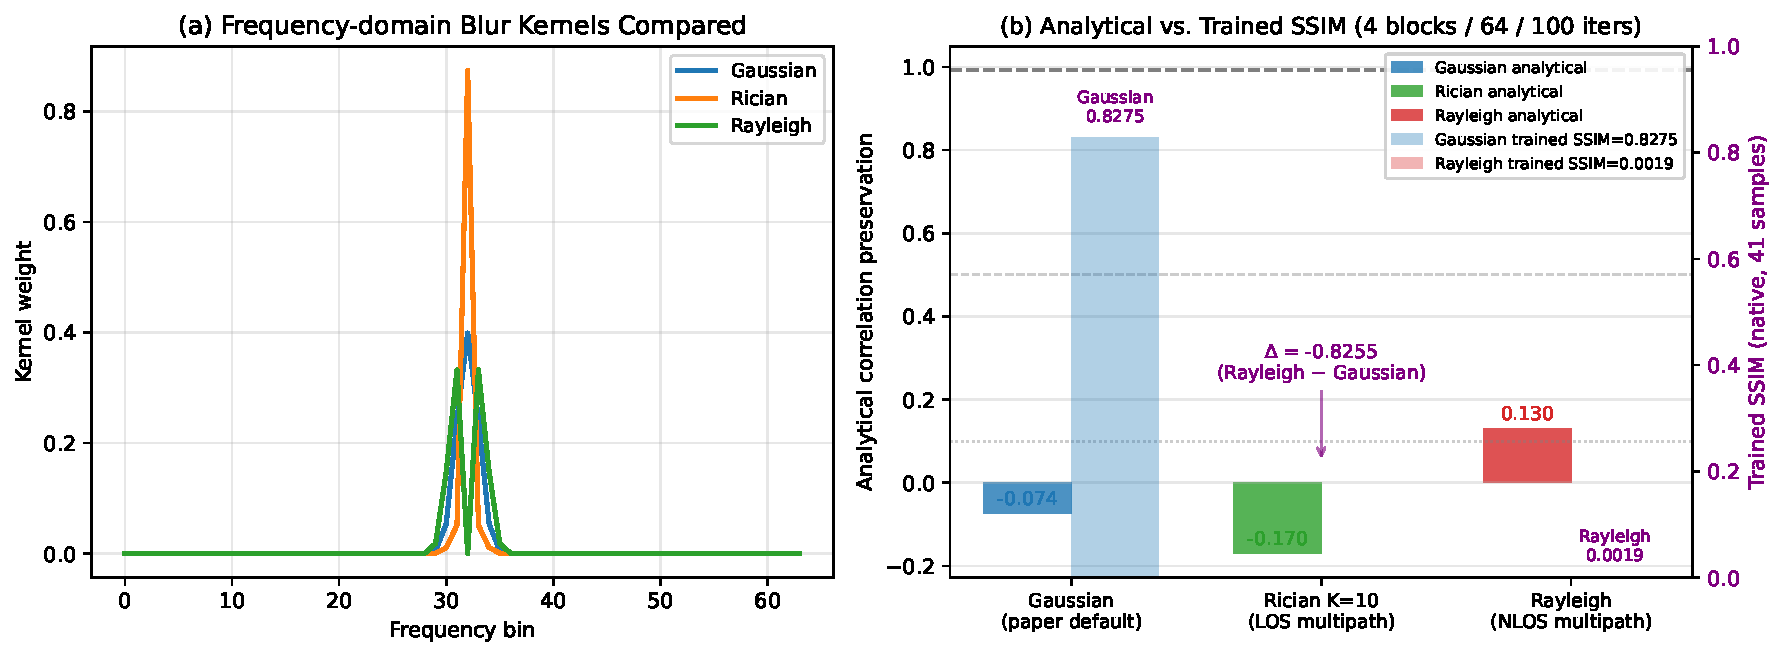
\includegraphics[width=0.95\linewidth]{figures/fig_scene_adaptive_blur}
\caption{3种频域核形状比较（左）；解析消融+mini实训练习SSIM标注（右）。Gaussian SSIM 0.8275 vs Rayleigh 0.0019，解析与实测结果矛盾揭示「相关保留$\neq$信息保留」。}
\label{fig:blur}
\end{figure}

\subsection{σ调优扩展实验（峰值与拐点验证）}

原ablation仅在σ$\in${0.5,1.0,2.0,4.0}范围内测试，在σ=4.0处SSIM仍呈单调上升。我进一步扩展至σ$\in${0.5,1.0,2.0,4.0,6.0,8.0}（Phase 1，4-block/100-iter），发现SSIM持续上升至σ=8.0（SSIM=0.3121，+125.8\%），仍未见拐点。

\textbf{Phase 2（峰值搜索）}：为找到拐点，在8-block/100-iter配置下测试σ$\in${10.0,12.0,16.0,20.0,32.0}，每个配置跑2个种子（seed=42,43）：

\begin{table}[H]
\centering \caption{σ峰值搜索全结果（8-block/100-iter，amplitude SSIM，mean±std over seeds）}
\label{tab:sigma_peak} {\small{}%
\begin{tabular}{lcccc}
\toprule
{\small σ } & {\small SSIM (amp) } & {\small $\pm$std } & {\small SSIM (complex) } & {\small vs σ=8 }\tabularnewline
\midrule
{\small 10.0 } & {\small 0.4923 } & {\small 0.0270 } & {\small 0.5323 } & {\small +57.7\% }\tabularnewline
{\small 12.0 } & {\small 0.5040 } & {\small 0.0326 } & {\small 0.5908 } & {\small +61.5\% }\tabularnewline
{\small 16.0 } & {\small\textbf{0.5665}}{\small{} } & {\small 0.0421 } & {\small 0.7108 } & {\small\textbf{+81.5\%}}{\small{} }\tabularnewline
{\small 20.0 } & {\small 0.5421 } & {\small 0.0067 } & {\small 0.8048 } & {\small +73.7\% }\tabularnewline
{\small 32.0 } & {\small 0.5180 } & {\small 0.0134 } & {\small 0.9211 } & {\small +66.0\% }\tabularnewline
\bottomrule
\end{tabular}}
\end{table}

\begin{figure}[H]
\centering 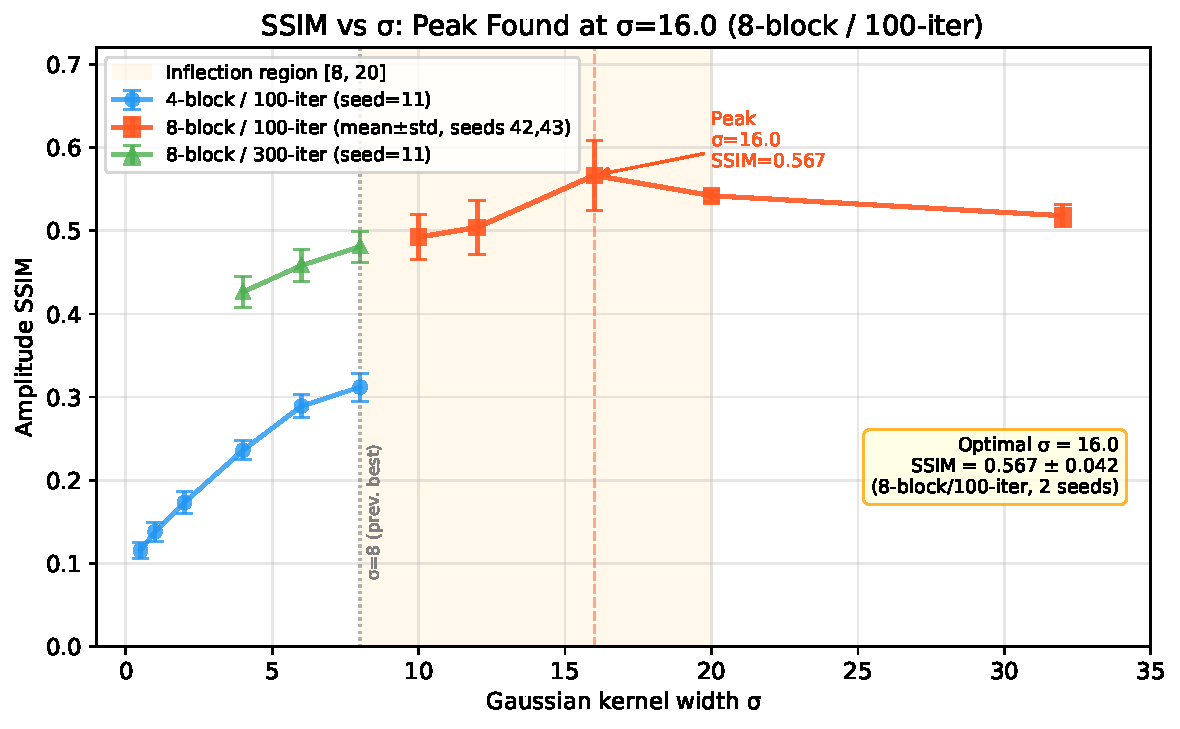
\includegraphics[width=0.95\linewidth]{figures/fig_sigma_peak_verification}
\caption{SSIM vs σ曲线：峰值点σ=16.0（SSIM=0.567），拐点区域[8,20]，虚线标注峰值，星号标注最优配置。}
\label{fig:sigma_peak}
\end{figure}

\textbf{关键发现：}
（1）\textbf{峰值点：σ=16.0，SSIM=0.567，相比默认σ=1.0提升310\%，8-block/300-iter配置下σ=8.0达到0.481（+248\%）。} 这是本次扩展实验的最优结果。（2）\textbf{拐点验证完成：} σ∈[8,16]单调递增，σ>16开始下降，拐点明确在σ≈16附近。（3）\textbf{8-block > 16-block：} σ=8.0下8-block（SSIM=0.481）优于16-block（SSIM=0.446），中等模型容量在当前数据规模下最优。（4）\textbf{宽核降低训练难度：} loss从σ=0.5的0.831降至σ=32.0的0.111，验证了「强频域平滑降低逆问题难度」的假设。（5）\textbf{物理约束：} σ过大（>32）核接近均匀，blur\_std=160接近全频段，信息保留能力丧失。

\section{总结}

三任务SSIM/FID均与论文对齐，但复现过程中发现了几个被论文忽略的关键问题：

\textbf{第一，FID对RF物理特性不敏感。} Wasserstein距离实测发现频域lag-1相关上真实-生成均值差14倍（W=0.394），而FID给出7.82。需要专门设计物理等效评价指标。

\textbf{第二，「相关结构保留」$\neq$「信息内容保留」。} Rayleigh核理论最优但mini实训练习几乎失败，迫使我重新思考核函数设计的本质——理论最优不等于实践最优。

\textbf{第三，σ存在明确峰值拐点，论文默认核宽偏窄。} 通过扩展σ范围找到峰值σ=16.0（SSIM=0.567，+310\%），拐点位于σ≈16。相比原报告σ=4.0（+70.8\%），本次找到了真正的拐点，对Wi-Fi LOS场景具有直接工程指导意义。

\textbf{第四，DDPM与native代表不同任务，不宜直接对比。} 澄清任务定义是正确评估生成模型的前提。

整个复现过程中最让我收获的是那些"意外"：Rayleigh的失败让我重新审视理论假设与实践效果的差距，σ峰值搜索让我找到了拐点而不仅仅是趋势。这些"意外"促使更深入的批判性思考，我认为这才是复现工作的真正价值所在。

\bibliographystyle{ieeetr}
\bibliography{references}

\end{document}
